\documentclass[10pt,a4paper,twocolumn]{jsarticle}
\bibliographystyle{jplain}
\setlength{\columnsep}{3zw}

%
\usepackage{amsmath,amssymb}
\usepackage{bm}
\usepackage[dvipdfmx]{graphicx}
\usepackage[dvipdfmx]{color}
\usepackage{ascmac}
\usepackage{here}
\usepackage{enumerate}
\usepackage{cases}
\usepackage{amsthm}
\usepackage{algorithm}
\usepackage{algorithmic}
\usepackage{lscape}
\renewcommand*{\proofname}{Solution}
%
\setlength{\textwidth}{1.1\fullwidth}
% \setlength{\textheight}{38\baselineskip}
\addtolength{\textheight}{\topskip}
\setlength{\hoffset}{-0.15in}
\setlength{\voffset}{-0.2in}
\setlength{\topmargin}{0pt}
\setlength{\headheight}{0pt}
\setlength{\headsep}{0pt}
%

\newcommand{\inputfig}[3]{
% Uncomment following line and delete the next to force figure to be in place of the command
\begin{figure}[H]
%\begin{figure}
    \centering
    \includegraphics[scale=#3]{./Figures/#1}
    \caption{#2}
    \label{fig:#1}
\end{figure}
}
\newcommand{\inputgraph}[3]{
% Uncomment this line and delete the next to force figure to be in place of the command
\begin{figure}[H]
%\begin{figure}
    \centering
    \resizebox{#3\hsize}{!}{\input{graphs/#1.tex}}
    \caption{#2}
    \label{graph:#1}
\end{figure}
}
\newcommand{\inputtable}[2]{
% Uncomment this line and delete the next to force table to be in place of the command
\begin{table}[H]
%\begin{table}
	\caption{#2}
	\label{table:#1}
	\centering
	\small
    \input{tables/#1.tex}
\end{table}
}
%


\title{Visual Scene Graph Extraction}
\author{中山研究室 修士一年 増井 建斗}
\date{\today}
\begin{document}
\maketitle

%========================================================================

\section{概要}
風景や物体などの一般的な環境を撮影した画像から,画像の内の情報をScene Graph\cite{scene_graph}と呼ばれるグラフ構造として出力するモデルを教師あり学習によって学習する方法を提案する.Scene Graphは画像内の情報を,物体とその属性のペアによるグラフ構造で表現したものである.教師あり学習に必要な画像とScene Graphは制作に多くの手間がかかり,学習に十分なデータ・セットが用意されていないため,コンピュータグラフィックスによって自動生成したデータ・セットを用いて学習を行う.また,Scene Graphを出力可能な機械学習モデルの提案を行う.
%========================================================================

\section{背景}
家庭内で家事を行うロボットの意思決定や画像検索においては,画像内の物体認識に加えて,それら物体同士の位置関係などの2物体以上に渡る関係性も重要な情報となる.従来の画像認識では画像内の物体のラベル付けと位置検出が行われているが,物体同士の関係性を含む情報を抽出する試みには,多くの研究余地が残されている.この研究の最終的な目標は,画像から物体同士の関係を含む情報を抽出することで家事ロボットによる意思決定を補助することであるが,画像検索などの問題にも適用可能である.

関連研究としてImage Retrieval using Scene Graphs\cite{scene_graph}があるが,彼らは検索対象の画像全てにScene Graphがあらかじめ作成されている前提で,自然言語による検索文と
Scene Graphのマッチングを行い高精度の画像検索を実現した.データセットの作成にはクラウドソーシングが利用され,全て人力でScene Graphが作成されている.この研究では画像からのScene Graphを行うモデルを教師あり学習するが,彼らが用意したデータセットより多くの教師データを用いるため,コンピュータ・グラフィックスによるデータセットの自動生成を行うこととした.
%========================================================================

\section{問題設定}
Scene Graphでは,画像内の情報を述語とその引数で表現する.例えば,Spoon,Cup,Tableが存在するとき,Cup on Tableという情報はOn(Cup,Table)のように表現され,Onが述語(Predicate),Cup,Tableがその引数(Parameter)である.述語と引数のペアを一つの事実(Fact)と呼ぶ.この時,述語をエッジ,引数をノードと解釈すると画像内の情報が事実の集合,グラフ構造で表現され,全体としては図\ref{fig:scene_graph}のように表現される.この研究では,画像からこのScene Graphを出力することを目標とする.
\inputfig{scene_graph}{シーングラフの例}{0.6}
\inputfig{dataset2}{レイトレーシングを用いて生成した学習用データセットの一部.一つの画像に2つの物体と1つの述語(関係)が含まれる.}{0.3}
この研究には3つの課題がある.一つは画像からの事実の抽出.もう一つは画像からのシーングラフの抽出.そして最後に学習に必要なデータセットの準備である.
3つの課題のうち,データセットについてはコンピューター・グラフィックス(CG)を用いてデータセットを作製することで解決することとした.残る2つの問題については,事実の抽出が可能であるかの検証を行ったうえで,シーングラフの抽出を目指すこととした.以降,データセットの作成と,事実の抽出,シーングラフの抽出について説明する.

%========================================================================

\begin{figure*}
%    \centering
\begin{center}
    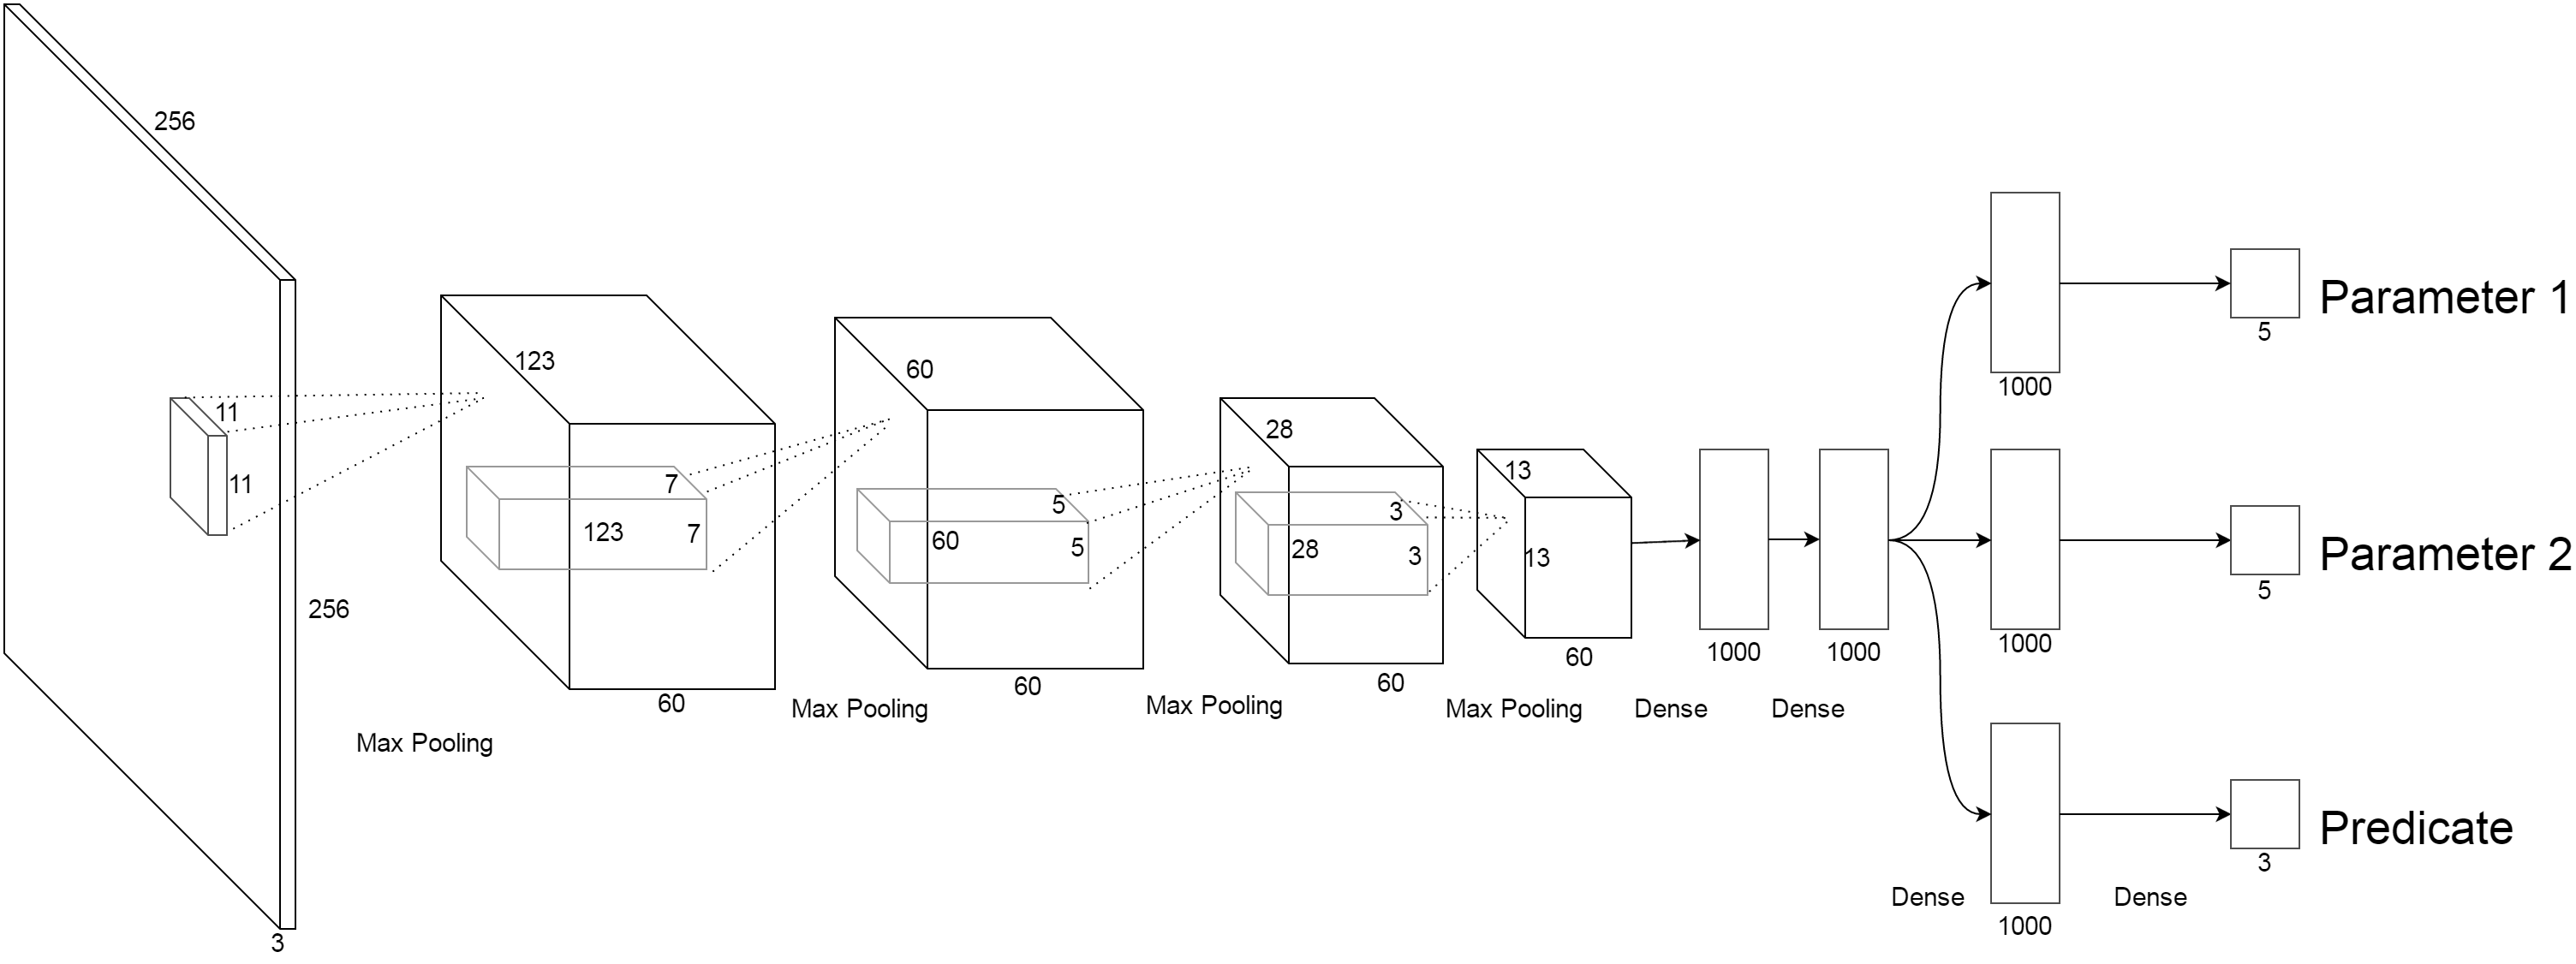
\includegraphics[scale=0.1]{./Figures/model1}
    \caption{事実抽出モデル}
    \label{fig:model1}
\end{center}
\end{figure*}
\section{データセットの作成}
以降で提案する教師あり学習モデルのため,大量に画像とScene Graphのペアを自動生成している.
図\ref{fig:dataset2}に,学習用データ・セットの一部を示す.

%========================================================================

\section{事実の抽出}
画像認識においては,畳込みニューラルネットワークが画像の特徴獲得に有効であることが確認されている.畳み込みニューラルネットワークは一般的には識別器と組み合わされ,画像の識別で高い精度を上げている.一般的な画像認識では一つの入力画像からその物体の種類を答えるが,今回は一つの事実を出力するために工夫が必要となる.図\ref{fig:model1}に,今回畳み込みニューラルネットワークをベースに作成した学習モデルを示す.
画像特徴量の抽出には一般的な畳込みニューラルネットワークを利用しているが,出力が三叉に分岐している.それぞれが2つの物体とその関係に対応している.この3つの出力を,一つの事実として解釈する。
この学習モデルを利用して事実の抽出を学習したところ,物体(述語引数)に関しては80から90\%以上の精度,物体間関係(述語)については95\%以上の精度で正解することができた.各物体の認識精度は図\ref{fig:p1_cm}のConfusion Matrixで確認することができる.
\inputfig{p1_cm}{事実抽出における物体認識精度を示すConfusion Matrix}{0.6}
%========================================================================
\section{シーングラフの抽出}
シーングラフの抽出では,複数の事実を出力させる必要がある.一つの入力から複数の時事を出力させるため,Long Short Term Memory (LSTM)\cite{lstm}を利用する.LSTMはニューラルネットワークの一種だが内部に状態を持ち,一回の出力ごとに内部状態を更新し可変長の出力が行える.一般的には自然言語処理等,前の出力が次の出力に影響を与える問題において力を発揮するが,今回はこの可変長出力部分を利用するために用いている.
\inputfig{model2}{シーングラフ抽出モデル}{0.4}

図\ref{fig:model2}にモデルの全体構造を示す.画像の入力からScene Graphの出力までの流れは,次のようになる.まず画像を幾層にも重ねられた畳み込みニューラルネットワークに入力し,その特徴表現を出力させる.次に,得られた特徴表現をLSTMに入力し,LSTMが終了記号を出力するまで,述語と引数のペアを出力させる.最終的に得られた述語と引数のペアの集合を,画像のScene Graphとする.
%========================================================================

\section{結論と今後の課題}
家事ロボットの行動決定に必要な画像内物体間関係認識に向けて,教師あり学習の枠組みで画像からScene Graphを出力するモデルを提案した.同時に,学習に必要なデータ・セットの作成を行った.事実の抽出可能性を示すことが出来たので,今後はシーングラフの抽出を目指し,データセットの拡充とともに提案手法の検討と比較を行う.
\bibliographystyle{plain}
\bibliography{./BibTeX/sample}
\end{document}
